\documentclass[conference]{IEEEtran}
\IEEEoverridecommandlockouts
% The preceding line is only needed to identify funding in the first footnote. If that is unneeded, please comment it out.
\usepackage{cite}
\usepackage{amsmath,amssymb,amsfonts}
\usepackage{algorithmic}
\usepackage{graphicx}
\usepackage{textcomp}
\usepackage{xcolor}
\usepackage[shortcuts,acronym]{glossaries}

\def\BibTeX{{\rm B\kern-.05em{\sc i\kern-.025em b}\kern-.08em
    T\kern-.1667em\lower.7ex\hbox{E}\kern-.125emX}}
    
\makeglossaries
\newacronym{api}{API}{Application Programming Interface}
\begin{document}

\title{Working Title - Transparency and Records of processing in agile DevOps:
Towards a GDPR-focused tracing Toolbox\\
{\footnotesize \textsuperscript{*}Note: Sub-titles are not captured in Xplore and
should not be used}
}

\author{
    \IEEEauthorblockN{Daniel Habenicht}
    \IEEEauthorblockA{\textit{Masters Student} \\
    \textit{TU Berlin}\\
    Berlin, Berlin \\
    email address or ORCID}
\and
    \IEEEauthorblockN{Lucas Kettenmann}
    \IEEEauthorblockA{\textit{Masters Student} \\
    \textit{TU Berlin}\\
    Berlin, Berlin \\
    email address or ORCID}
\and
    \IEEEauthorblockN{Piotr Witkowski}
    \IEEEauthorblockA{\textit{Masters Student} \\
    \textit{TU Berlin}\\
    Berlin, Berlin \\
    email address or ORCID}
}

\maketitle





\begin{abstract}
Blala lal This and the IEEEtran.cls file define the components of your paper [title, text, heads, etc.]. *CRITICAL: Do Not Use Symbols, Special Characters, Footnotes, 
or Math in Paper Title or Abstract.
\end{abstract}

\begin{IEEEkeywords}
component, formatting, style, styling, insert
\end{IEEEkeywords}

\section{Introduction}
This document is a model and instructions for \LaTeX.
Please observe the conference page limits. 

\section{Prerequisites}

\subsection{Legal requirements and the principle of transparency}
% Briefly sketch the “privacy principle“ you are about to address with your semester subject (legal grounding is highly welcome)  

% Interesting Link: https://www.i-scoop.eu/gdpr/legal-grounds-lawful-processing-personal-data/
% privacy by transparency art12ff + (evtl. 30??)
% legal ground citations fron gdpr, table from \cite{ErnstTransparencyComputing} extend for location and more detailed description of data we want to collect
% GDPR legal grounding social aspects? 
% name his favourite sentence "if this tech will get mainstream it will be required by law"
% Other legal grounds: California? USA? other 
% Lesson 3: why privacy is a "blurry" concept, "abstract" goals, what societally agreed upon as necessary / helpful principles are 

A main reason for the necessity of new approaches and tools regarding privacy is the General Data Protection Regulation (GDPR) which became effective in May 2018. Still to this day many companies struggle to adhere to this regulations, which opens up both challenges and chances.

The GDPR regulates the processing of personal data ("'personal data' means any information relating to an identified or identifiable natural person", GDPR Art. 4(1)) \cite{EuropeanParliamentandoftheCouncil3026GeneralRegulation}). In such it differs between the natural person whose data is processed, also called the "data subject", and the entity which " determines the purposes and means of the processing of personal data" (GDPR Art. 4(7) \cite{EuropeanParliamentandoftheCouncil3026GeneralRegulation} as "controller". The "processor" is the entity which does the actual processing of the 
data on behalf of the controller (GDPR Art. 4(8)) \cite{EuropeanParliamentandoftheCouncil3026GeneralRegulation}.

Art. 12-15 of the GDPR require that all the personal data of a data subject including the reasons to process it (GDPR Art. 13(1d), 14(2b) as well as the processed data itself (GDPR Art. 15(3, 4)\cite{EuropeanParliamentandoftheCouncil3026GeneralRegulation}) are to be provided to the data subject by the controller. Furthermore it is necessary for a controller to "maintain a record of processing activities under its responsibility" (GDPR Art. 30(1) \cite{EuropeanParliamentandoftheCouncil3026GeneralRegulation}).

The above mentioned articles are part of the principle of transparency (GDPR Art. 5(1) \cite{EuropeanParliamentandoftheCouncil3026GeneralRegulation}) which assumes that the controller is clearly stating the processed data it's purpose to the data subject. To accumulate this data the controller needs to be aware of all components in a system which are conduction data processing of personal data and the purpose of the processing. A solution for this problem will be presented by this paper.


\subsection{Problem definition}\label{problem}

% Describe current setting (top-down GDPR policies) and current development practices (agile) expressing the need for a better (our) solution
% Different Domains clashing ( Developer <> Data Privacy Law (Jura))
% \cite{ErnstTransparencyComputing} only on service level but reasons should be give more fine grained (e.g. monolithic architecture, not everything is processed with the same purpose
% otherway around data types are the same in a system this don't have to be redefined for each service)

A straightforward approach for tracing the personal data which is collected and processed by a system with privacy in mind would be top-down. Different systems are identified and manually evaluated for GDPR relevant user data. Rather time intensive processes for the identification and cataloguing of this data are required, and even if those processes are well-defined and carried out with utmost diligence the risk of overlooking certain data in complex systems is high.

As systems change, this data needs to be kept up-to-date. In recent years agile development approaches have become more and more common, such as Scrum, Kanban or Extreme Programming. Clustered, rather independent teams change individual system components multiple times a week or even a day while automated processes verify the system integrity. This opens up the opportunity for automated tracing of the processing of privacy related data and it's adherence to the privacy principles required by the GDPR. Obviously, the top-down approach to privacy is not feasible in the context of small, dispersed teams and rapidly changing systems with many independent components.

A bottom-up approach, where data is identified from within the system components themself, can facilitate the process of maintaining a database of handled user data. This would require every developer of a system or system component to report the privacy-related data which is processed by it to a central site. This process requires a considerable amount of work, especially in larger companies with non streamlined processes and clustered competences. In a real-world scenario it is unrealistic to assume that every developer of a large system will accurately report any user data his components are using. An automated approach to this will mitigate the human weak point and standardize it to achieve consistent results by embedding the report functionality into the system as a mandatory part of the communications protocol. By linking every packet of data to it's purpose in terms of privacy and the GDPR all user data in the system becomes traceable. As such a system-wide analysis can be conducted and the data can be made available condoning to the principle of transparency.

\section{Tech}

\subsection{Analysis and viability of technologies}
%  Which tech do we use? What is it? 
% Identify and technically describe available technologies that might be used (if any)

Applying the \ac{gdpr} becomes especially difficult when data is transferred from one system to another. The most common \ac{api} Standard in between services is \ac{rest}, which is used for over 80\% \cite{CloudElements2017TheIntegration} of the \glspl{api} in 2017. In order to document \ac{rest} \glspl{api} multiple standards emerged, for example API Blueprint, I/O Docs, Swagger, RAML, WADL and WSDL \cite{Scherer2016DescriptionTransformation}. The general standard nowadays is the \ac{oas}, which emerged from the Swagger Standard. OpenAPI was ranked as the fourth most important technology for people working with \glspl{api} \cite{2019Technologies2019}. 

\begin{quote}
"The OpenAPI Specification defines a standard, programming language-agnostic interface description for REST APIs, which allows both humans and computers to discover and understand the capabilities of a service without requiring access to source code, additional documentation, or inspection of network traffic. [\dots]"
\cite{OpenAPISpecification}
\end{quote}

Most of the previously named standards are providing migrations or compatibility to the OpenAPI standard \cite{Scherer2016DescriptionTransformation}.
% https://github.com/oasis-tcs/odata-openapi


It is supported by the OpenApi initative, which is joined by major companies like Microsoft, Google, \cite{TheLinuxFoundation2020CurrentInitiative}
The standard developed from the Swagger Specification and is now almost 9 years old. 

OpenAPI is partly based on JSON Schema language which describes JSON Payload 



\begin{figure}[htbp]
\centerline{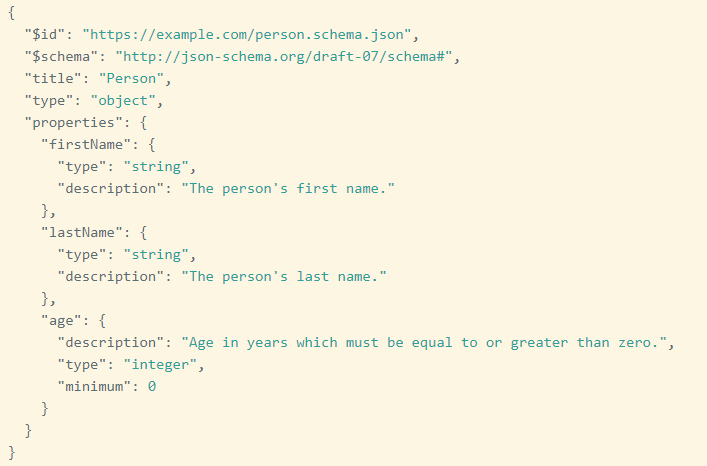
\includegraphics[width=0.4\textwidth]{figures/json_schema_example.png}}
\caption{Example of Json Schema used in OpenAPI \cite{MiscellaneousSchema}}
\label{json_schema_example}
\end{figure}

JSON Schema also allows to "outsoure" the assessment of data categories to professionals. 




For our prototype we are using NodeJS Services

based on Express 

Javascript/Typescript Language for object oriented programmming which provides both typed experience and untyped functions. This will speed up and make. 

As the prototype will not reach production status we do no not need to factor in runtime performances. 

\subsection{Short Introduction to Technologies}




% explain OpenAPI (maybe some history of swagger as well, but not too lengthy) 
% maybe the differences between Swagger(v2) and OpenAPI(v3)? JSONSchema 
% Computer-readable format is needed to be make automated (or semi-automated) processing possible -> OpenAPI is a standard allowing us to describe APIs
% explain tracing frameworks like Zipkin and Jaeger
% explain static analysis
% runtime variables in cloud, eg. location (AWS has variables) 

% Assess practical viability of said technologies

% formulate why we used static analysis or tracing frameworks and which tradeoffs these have
% maybe some usage statistics about OpenAPI / tracking / other tools? How many developers are using it? Is it easy to implement? 
% Why these solutions? What are alternatives and why did we not choose them? 
% Ranking of Tools? 
% How much effort is it? 

% OpenAPI is very versatile: Code can be annotated to generate the specification, but there are also Code generation solutions that generate code from the spec itself.


\subsection{Prototype}
% Provide a (sketchy) outlook about what you are going to implement (esp. your re-usable component)

As described in section \ref{problem} we want to make it easier to track data throughout multiple applications and make it more clear for which purposes . 
We based this on defining the type of data in a central place, which we identiefied as OpenAPI. In order to track data inside of the application we also need a service middleware, which enriches a request with the legal context and logs the type of data transferred. 
Collecting the 
Our Prototype will be set up in a business context. It will simulate a sleep tracking app. Which collects different categories of personal data for different purposes, while being based on a micro-service architecture. 

It will roughly look like the system shown in Figure \ref{prototype_system}

\begin{figure}[htbp]
\centerline{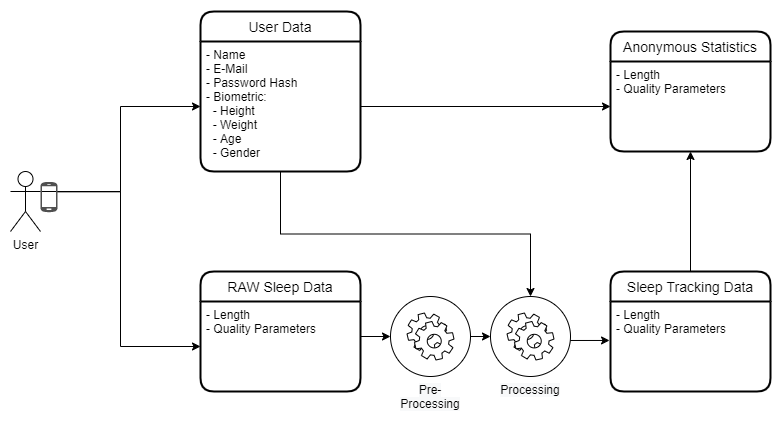
\includegraphics[width=0.4\textwidth]{figures/prototype_system.png}}
\caption{Sketch of our prototype system}
\label{prototype_system}
\end{figure}

Our reusable software components can be split into three main areas: 

\begin{itemize}
    \item Schema Specifications
    \item Service Middleware 
    \item Data collector and analyzer 
\end{itemize}



This could be extended by providing decorators for easier schema specifactions or visualizations for the output data. 
% - Diagramm sketch 
% - flow diagram 

% - Reusable Component: 
%    - OpenAPI Specification based on "Transparency Tracing v2"
%    - Middleware for adding purpose to requests 
%       https://rhonabwy.com/2019/01/06/adding-tracing-with-jaeger-to-an-express-application/
%    - Linter for checking those: https://palantir.github.io/tslint/develop/custom-rules/
%     % https://medium.com/@andrey.igorevich.borisov/writing-custom-tslint-rules-from-scratch-62e7f0237124
%    - Zero Config - Middleware -> % should log to localhost by default? 
    % https://expressjs.com/en/guide/writing-middleware.html
    
    
%    - Visualization of said trace 
%    - Decorator pattern for adding specification easily to OpenAPI % and enable logging itself?
%    - static analysis tool for tracing the data flow

Goals: 

While building a prototype we think that while making something technically feasible it is even more important to make it useful and easily usable. 

Address that services are mostly not microservices in the sense of they fulfill only one purpose (in a GDPR sense) but are fulfilling multiple purposes. e.g. a (example from our system) This has to be taken care of at the application level, for each data request) 

Another pain point is the manual work needed to work with frameworks like yappl which defines a "privacy proxy" which policies assume that the requesting service sends required data like "Institution or Service Name" and "Purpose" in order to enforce the user decision. In future version this could also be extended to related datapoints like "processing-location" "legal-base (and legitimate-interest)" "data-categories" "storage-ttl" "automted-decision-making" \dots .
To this, at the moment the developer has to write and update these strings manually. With out proposed solution this could be partly auto generated.
 
 
 Our approach takes the baseline implementation of \cite{ErnstTransparencyComputing} and updates it to be request specific, while maintaining developer comfort to failback to the centrally provided values. We do this because 
 Because this would lead to the same status quo as before, as nobody would use the optional configuration options we propose a set of easy linting rules which can be applied to each request and inform about more detailed GDPR infos. Another option would be to implement yet another request library to make these required. But in the light of the multitude of availabe languages and the tools available for each language we find that linting rules provide the best approach to be easily rewritten for each tool. 
 The Linter will be based on TSLint which is the standard Linting tool for typescript. 
 
 
 In order to fallback the 
 
 For analyzing purposes we first thought of a static analysis. But this would have several limits. e.g. the used servers (database etc.) are mostly configured at runtime in the production environment. 


Because implementing a Tracing Middleware for each request we might resort to a simpler self-written middleware or mock the responses for the analyzation step. 

During the design of our prototype our subgoal is to not hinder productivity of the developer. 
As this is one of the main pain points in current development \cite{StateDevOps}. 


\printglossaries

\bibliographystyle{IEEEtran}
\bibliography{references}


\end{document}
